Let $a(x), b(x) \in \mathcal{R}$ be two polynomials. To calculate the product $c(x) = a(x)\cdot b(x)$ the most straightforward
approach, also known as the \emph{schoolbook} algorithm, consists in multiplying each monomial of the first with each monomial of the second,
add together the results of the same degree and reduce the result modulo $x^n-1$. With this method we can calculate the product of the polynomials with $\mathcal{O}(n^2)$ multiplications
and $\mathcal{O}(n^2)$ additions, as the degree of the operands is at most $n-1$. Even though this approach is simple to understand and implement, 
it does not scale well as the degree of the operands increases: for this reason, other multiplication algorithms have been proposed.

As shown by Bernstein in~\cite{bernstein2001multidigit}, we can think of most of the polynomial multiplication algorithms in the literature
as follows:
\begin{itemize}
    \item \textbf{Lifting} the operands to different rings via a ring homomorphism $f$
    \item Multiplying the lifted polynomials in the ring
    \item \textbf{Mapping} the result back to the original ring via the inverse homomorphism $f^{-1}$
\end{itemize} 
By carefully choosing the destination ring and the homomorphism, we can obtain algorithms with drastically better asymptotic complexity:
in the remainder of this section we will discuss two of the most common algorithms, Karatsuba and the Fast Fourier Transform. 

\subsection{Karatsuba multiplication}
The Karatsuba algorithm~\cite{karatsuba1962multiplication} is a divide and conquer algorithm that splits a $n$-degree polynomial into 
two $n/2$-degree polynomials and then calculates the product of the original polynomials in $\mathcal{O}(n^{\log_2 3})$ operations.

Starting from $a(x)$, $b(x)$ of degree $n$ and an integer $m < n$, we can write
\begin{equation*}
\begin{aligned}
    a(x) &= a_0(x) + x^m\cdot a_1(x) \\
    b(x) &= b_0(x) + x^m\cdot b_1(x)
\end{aligned}
\end{equation*}
where $a_0(x)$ and $b_0(x)$ have degree less than $m$. This split is valid for any positive $m < n$, but in order to achieve the
aforementioned complexity we split the inputs into equal parts.

At this point, we can calculate the product $c(x) = a(x)\cdot b(x)$ as
\begin{equation*}
    \begin{aligned}
        c(x) &= a(x)\cdot b(x) \\
             &= (a_0(x) + x^m\cdot  a_1(x))\cdot (b_0(x) + x^m\cdot  b_1(x)) \\
             &= a_1(x)\cdot b_1(x)\cdot x^{2m} + (a_1(x)\cdot b_0(x) + a_0(x)\cdot b_1(x))\cdot x^m + a_0(x)\cdot b_0(x)\\
             &= z_2(x)\cdot x^{2m} + z_1(x)\cdot x^m + z_0(x)
    \end{aligned}
\end{equation*}
where
\begin{equation*}
    \begin{aligned}
        z_2(x) &= a_1(x)\cdot b_1(x) \\
        z_1(x) &= a_1(x)\cdot b_0(x) + a_0(x)\cdot b_1(x) \\
        z_0(x) &= a_0(x)\cdot b_0(x)
    \end{aligned}
\end{equation*}
Karatsuba observed that, at the cost of some few additions, we can calculate $a(x)b(x)$ with three multiplications by rewriting $z_1$ as
\begin{equation*}
    z_1(x) = (a_0(x) + a_1(x))\cdot (b_0(x) + b_1(x)) - z_0(x) - z_2(x)
\end{equation*}

\begin{example}[Karatsuba multiplication]
From the ring of binary polynomials $\mathcal{R}$ we take $a(x) = 1 + x + x^3$ and $b(x) = x + x^2$; by choosing $m=2$, we rewrite the operands as
\begin{equation*}
    \begin{aligned}
        a(x) &= (1+x) + x^2\cdot (x)\\
        b(x) &= (x) + x^2\cdot (1)
    \end{aligned}
\end{equation*}
and calculate the subproducts as
\begin{equation*}
    \begin{aligned}
        z_2(x) &= (1+x)\cdot (x) = x + x^2 \\
        z_0(x) &= (x)\cdot (1) = x \\
        z_1(x) &= (1+x + x)\cdot (x + 1) - (x) - (x+x^2) = 1 + x + x^2
    \end{aligned}
\end{equation*}
From the above, we can calculate the full product as
\begin{equation*}
    \begin{aligned}
        c(x) &= (x)\cdot x^{2\cdot 2} + (1 + x + x^2)\cdot x^2 + (x+x^2) \\
             &= x^5 + x^4 + x^3 + x
    \end{aligned}
\end{equation*}
\end{example}

The input polynomials can be split into an arbitrary amount of parts, and the product calculated in a similar fashion:
such a product is calculated by the Toom-Cook algorithm~\cite{cook1969minimum}, which is a generalization of Karatsuba's algorithm.

\subsection{Fast Fourier Transform}

We can approach polynomial multiplication in a totally different way. Instead of multiplying the polynomial coefficients, we can
evaluate the inputs at a set of points (\emph{sampling}) and, for each pair of samples $a(i), b(i)$, calculate the pointwise product
$c(i) = a(i)\cdot b(i)$. By performing this operation $2n+1$ times, where $n$ is the maximum degree of the input polynomials, the interpolation
theorem guarantees that the (unique) polynomial that interpolates the samples $c(i)$ is the product of the original polynomials.
\begin{example}
    Let $a(x) = x^2 + 2x + 3$ and $b(x) = 4x + 5$ be polynomials with real coefficients of degree at most $n=2$; since their product
    will have degree at most $2n=4$ we evaluate the polynomials at $2n+1$ points:
    \begin{align*}
        a(0) = &1\cdot 0^2 + 2\cdot 0 + 3 = 3 \quad &b(0) = &0\cdot 0^2 + 4\cdot 0 + 5 = 5 \\
        a(1) = &1\cdot 1^2 + 2\cdot 1 + 3 = 6 \quad &b(1) = &0\cdot 1^2 + 4\cdot 1 + 5 = 9 \\
        a(2) = &1\cdot 2^2 + 2\cdot 2 + 3 = 11 \quad &b(2) = &0\cdot 2^2 + 4\cdot 2 + 5 = 13 \\
        a(3) = &1\cdot 3^2 + 2\cdot 3 + 3 = 18 \quad &b(3) = &0\cdot 3^2 + 4\cdot 3 + 5 = 17 \\
        a(4) = &1\cdot 4^2 + 2\cdot 4 + 3 = 27 \quad &b(4) = &0\cdot 4^2 + 4\cdot 4 + 5 = 21 \\
        %a(5) = &1\cdot 5^2 + 2\cdot 5 + 3 = 38 \quad &b(5) = &0\cdot 5^2 + 4\cdot 5 + 5 = 25 \\
    \end{align*}
    We can then calulate the pointwise multiplication of the samples
    \begin{align*}
        c(0) = &a(0)\cdot b(0) = 3\cdot 5 = 15 \\
        c(1) = &a(1)\cdot b(1) = 6\cdot 9 = 54 \\
        c(2) = &a(2)\cdot b(2) = 11\cdot 13 = 143 \\
        c(3) = &a(3)\cdot b(3) = 18\cdot 17 = 306 \\
        c(4) = &a(4)\cdot b(4) = 27\cdot 21 = 567 \\
        %c(5) = &a(5)\cdot b(5) = 38\cdot 25 = 950 \\
    \end{align*}
    Finally, we can interpolate the result to obtain the coefficients of the product:
    \begin{equation*}
        c(x) = 4x^3 + 13x^2 + 22x + 15
    \end{equation*}
\end{example}
This approach might appear slower than the schoolbook method: the sampling requires $\mathcal{O}(n^2)$ operations, the pointwise product
$\mathcal{O}(n)$ and the interpolation up to $\mathcal{O}(n^3)$ if we use a naive method such as Gaussian elimination; however, 
with the right choice of sampling points, we can drastically reduce the operations required in all three steps.

Instead of sampling at $N = 2n+1$ random points, we can choose the points to be the $N$-th roots of unity, \textit{i.e.} the points
$\omega_k = e^{-\frac{2\pi ik}{N}}$ for $k=0,\dots,N-1$. By writing the polynomial as a sum with coefficients $x_i$, the sampling at the $N$-th roots of unity
can be written as
\begin{equation}
    \mathcal{F}(\omega_k) = \sum_{n=0}^{N} x_n e^{-\frac{2\pi ik}{N}n}
    \label{DFT}
\end{equation}
which corresponds to the Discrete Fourier transform (DFT) of the polynomial.

At this point we can perform the pointwise product in the \textit{transformed} domain.
Once we get the samples $X_k$, we would have to interpolate them to get the coefficients of the product polynomial; however,
Parseval's theorem ties the sequences of samples ($x_n, y_n$) and their DFTs ($X_n, Y_n$) as in the following equation:
\begin{equation}
    \sum_{n=0}^{N} x_n\cdot y_n^* = \frac{1}{N}\sum_{k=0}^{N} X_k\cdot Y_k^*
\end{equation}
\newpage
Therefore, since the DFT is invertible, we can apply the inverse DFT to the samples $X_k$ to get the coefficients of the product polynomial:
\begin{equation}
    \mathcal{F}^{-1}(X_k) = \frac{1}{N}\sum_{n=0}^{N} X_n e^{\frac{2\pi i k}{N}n}
\end{equation}

The algorithms that compute the Discrete Fourier Transform of a sequence (or its inverse) are called Fast Fourier transforms (FFTs), and have an asymptotic complexity
of $\mathcal{O}(n\log n)$ for $n$ a power of 2; in case this last condition is not met, the inputs are padded with zeros to the next power of 2 in order to
achieve the same complexity.

\subsubsection{Cooley-Tukey FFT}
The Cooley-Tukey FFT~\cite{cooley1965algorithm} is the most common FFT algorithm. It is a \textit{divide et impera} algorithm, which recursively expresses a DFT of
size $N = N_1 N_2$ into $N_1$ smaller DFTs of size $N_2$ each. The simplest form of the Cooley-Tukey algorithm is the radix-2 decimation-in-time FFT, which 
splits a size-$N$ DFT into two size-$N/2$ smaller DFTs, interleaving odd and even-indexed inputs. 
Assuming that N is a power of 2, we can rewrite the DFT as:
\begin{align*}
    X_k & = \sum_{n=0}^{N-1} x_n e^{-\frac{2\pi i}{N}nk} \\
        & = \sum_{m=0}^{\frac{N}{2}-1}x_{2m}e^{-\frac{2\pi i}{N}(2m)k} + \sum_{m=0}^{\frac{N}{2}-1}x_{2m+1}e^{-\frac{2\pi i}{N}(2m+1)k} \\
        & = \sum_{m=0}^{\frac{N}{2}-1}x_{2m}e^{-\frac{2\pi i}{\frac{N}{2}}mk} + e^{-\frac{2\pi i}{N}k}\sum_{m=0}^{\frac{N}{2}-1}x_{2m+1}e^{-\frac{2\pi i}{\frac{N}{2}}mk} \\
        & = E_k + e^{-\frac{2\pi i}{N}k}O_k \qquad \text{ for } k = 0, \cdots, \frac{N}{2}-1
\end{align*}
where $E_k$ and $O_k$ group the evaluations of the even and odd-indexed input coefficients, respectively.

Because of the periodicity of the complex exponential, we can also write:
\begin{align*}
    X_{k+\frac{N}{2}} & = \sum_{m=0}^{\frac{N}{2}-1}x_{2m}e^{-\frac{2\pi i}{\frac{N}{2}}m(k+\frac{N}{2})} + e^{-\frac{2\pi i}{N}(k+\frac{N}{2})}\sum_{m=0}^{\frac{N}{2}-1}x_{2m+1}e^{-\frac{2\pi i}{\frac{N}{2}}m(k+\frac{N}{2})} \\
        & = \sum_{m=0}^{\frac{N}{2}-1}x_{2m}e^{-\frac{2\pi i}{\frac{N}{2}}mk}e^{-2\pi mi} + e^{-\frac{2\pi i}{N}k}e^{-\pi i}\sum_{m=0}^{\frac{N}{2}-1}x_{2m+1}e^{-\frac{2\pi i}{\frac{N}{2}}mk}e^{-2\pi mi} \\
        & = \sum_{m=0}^{\frac{N}{2}-1}x_{2m}e^{-\frac{2\pi i}{\frac{N}{2}}mk} - e^{-\frac{2\pi i}{N}k}\sum_{m=0}^{\frac{N}{2}-1}x_{2m+1}e^{-\frac{2\pi i}{\frac{N}{2}}mk} \\
        & = E_k - e^{-\frac{2\pi i}{N}k}O_k \qquad \text{ for } k = 0, \cdots, \frac{N}{2}-1
\end{align*}
This means that we can express a DFT of size $N$ as two DFTs of size $N/2$; moreover, we can re-use intermediate results to calculate multiple outputs,
as the roots of unity are the same for both DFTs and the complex exponential is periodic ($-\omega^k = \omega^{k+\frac{N}{2}}$). 
Since the base case of the recursion has complexity $\mathcal{O}(n)$ we get the recurrence relation $T(n) = 2T(\frac{N}{2}) + \mathcal{O}(n)$;
following the Master theorem~\cite{bentley1980general}, the computational complexity of the Cooley-Tukey FFT is $\mathcal{O}(n\log n)$.


\subsection{Additive FFT}
    The Cooley-Tukey FFT works when the $n$ points to sample are $n$-th roots of unity, and hence form a cyclic multiplicative group;
    this and similar algorithms are also referred to as \textit{multiplicative} FFTs, as they are based on the factorization of $x^n-1$.\\
    Unfortunately, multiplicative FFTs do not work when the underlying field does not admit non-trivial primitive roots of unity, as it happens for fields
    of characteristic two; for this reason, \textit{additive} FFTs were invented~\cite{DBLP:journals/jsac/WangZ88,DBLP:journals/jct/Cantor89}.
    Instead of using the $n$-th roots of unity, additive FFTs evaluate the polynomials at the powers of a primitive element of the field,
    as well as the zero element. Some examples of such algorithms that work on binary fields are the Gao-Mateer FFT~\cite{DBLP:journals/tit/GaoM10} 
    and the Lin-Chung-Han FFT~\cite{DBLP:conf/focs/LinCH14}, which perform similar procedures but require different representations for the polynomials.\\
    We will now focus on the LCH FFT, as it will be the foundation for a faster approach based on the Frobenius map; for this reason, we will
    consider the case $n=2^m$ where $m$ is a power of 2.
    
    \subsubsection{Cantor basis}
    In~\cite{DBLP:journals/jct/Cantor89} Cantor showed how to get a special basis for  the vector space $\mathds{F}_2^m$ in which it is possible to compute the FFT efficiently
    for any $m = p^n$, with $p$ a prime number; later in~\cite{DBLP:journals/tit/GaoM10} Gao and Mateer used a simpler construction for the special case
    $p=2$, where the Cantor basis $\mathbf{v} = (v_1, \cdots, v_{m})$ of $\mathds{F}_2^m$ follows the structure:
    \begin{equation}
        v_1 = 1, \quad v_i^2+v_i = v_{i-1} \text{ for } i > 1
    \end{equation}
    With respect to the Cantor basis $\mathbf{v}$, we define its sequence of subspaces of $\mathds{F}_2^m$ as:
    \begin{equation}
        \mathbf{W}_0 := \{0\}, \quad \mathbf{W}_i := span\{v_0, \cdots, v_{i-1}\} \text{ for } i \geqslant 1
    \end{equation}

    By construction, we have that $\mathbf{W}_0 \subset \mathbf{W}_1 \subset \cdots \subset \mathbf{W}_{m-1} = \mathds{F}_{2^m}$ 
    and the basis for a smaller space is contained into the basis of a larger space: this means that 
    we can arbitrarily treat elements of smaller fields as elements in the larger fields by padding zeros to the extra dimensions.

    With respect to each element of the basis $v_i$ we can define its subspace polynomial $s_i(x)$, also called vanishing polynomial, as:
    \begin{equation}
        s_i(x) = \prod_{a \in \mathbf{W}_i} (x - a)
        \label{eq:vanishing_polynomial}
    \end{equation}
    Since $\dim(\mathbf{W}_i) = i$ we have $\deg(s_i(x)) = |\mathbf{W}_i| = 2^i$.
    The vanishing polynomials, as shown in~\cite{DBLP:journals/jct/Cantor89,DBLP:journals/tit/GaoM10}, satisfy the following useful properties:
    \begin{itemize}
        \item linearity: $s_i(x+y) = s_i(x) + s_i(y)$
        \item recursivity: $s_{i+j}(x) = s_i(s_j(x))$ or, equivalently, $s_{i+1}(x) = s_i(x)^2+s_i(x)$
        \item $s_i(v_i) = 1$, for $v_i$ in the Cantor basis (see~\cite{DBLP:journals/corr/abs-1708-09746}, Appendix A for the proof)
        \item the roots of $s_i(x)$ are the elements of $\mathbf{W}_i$
    \end{itemize}
    Note that $\mathbf{W}_i$ is also a field whenever $i$ is a power of two; in that case, the vanishing polynomial has the form $s_i(x) = x^{2^i}+x$.

    \begin{example}[Cantor basis in $\mathds{F}_{16}$]
        Recalling that $GF(16) = GF(2)[x]/\langle X^4+X+1 \rangle$ and that $v_1 = 1$, we can compute $v_i = \beta(1) + \gamma(x) + \delta(x^2) + \epsilon(x^3)$,
        where the coefficients can be found by solving:
        \begin{equation*}
            \beta(1+1^2)+\gamma(x+x^2) + \delta(x^2+(x^2)^2) + \epsilon(x^3+(x^3)^2) = v_{i-1}
        \end{equation*}
        
        The resulting Cantor basis is $\mathbf{v} = (1, \alpha+\alpha^2, \alpha, \alpha+\alpha^3)$, inducing the subspaces $\mathbf{W}_i$:
        \begin{itemize}
            \item $\mathbf{W}_0 = \{0\}$
            \item $\mathbf{W}_1 = \{0, 1\}$
            \item $\mathbf{W}_2 = \{0, 1, \alpha+\alpha^2, 1+\alpha+\alpha^2\}$
            \item $\mathbf{W}_3 = \{0, 1, \alpha+\alpha^2, 1+\alpha+\alpha^2, \alpha, 1+\alpha, \alpha^2, 1+\alpha^2\}$
            \item $\mathbf{W}_4 = \mathds{F}_{16}$
        \end{itemize}
    Consequently, the vanishing polynomials are:
    \begin{itemize}
        \item $s_0(x) = x$
        \item $s_1(x) = x+x^2$
        \item $s_2(x) = x^4+x$
        \item $s_3(x) = x^8+x^4+x^2+x$
        \item $s_4(x) = x^{16}+x$
    \end{itemize}
    \end{example}

    \paragraph{A \textit{novel} polynomial basis}
    In order to perform the LCH FFT, the input polynomial has to be represented in a different basis. Given the Cantor basis $\mathbf{v} = (v_1, \cdots, v_m)$, we define the 
    \emph{novelpoly} basis with respect to $\mathbf{v}$ as $(X_1, \cdots, X_{n-1})$, defined as follows:
    \begin{equation}
        X_k(x) = \prod(s_i(x))^{b_i} \qquad \text{ where } k = \sum_{i=0}^{\log_2 n} b_i 2^i
    \end{equation}

    \begin{algorithm2e}[H]
        \caption{Basis conversion from monomial to \emph{novelpoly}}
        \label{alg:basiscvt}
        \KwIn{$f(x) = f_0 + f_1x+f_2x^2+\cdots + f_{n-1}x^{n-1}$, binary polynomial in canonical basis}
        \KwOut{$g(X) = g_0 + g_1X_1(x) + g_2X_2(x) + \cdots + g_{n-1}X_{n-1}(x)$, the representation of $f(x)$ in \emph{novelpoly} basis}
        \KwData{$y = x^{2^i}+x = s_i(x)$, the $i$-th vanishing polynomial}
        \SetKwFunction{BasisCvt}{\textsc{BasisCvt}}
        \SetKwProg{Fn}{Function}{}{}

        \Fn{\BasisCvt{$f(x)$}}{
            \If{$\deg f(x) \leqslant 1$} {
                \KwRet{$g(X) \gets f_0 + f_1X_1$}\;
            }
            $i \gets \max(2^k)$ s.t. $\deg(s_i(x)) \leqslant \deg(f(x))$\;
            $\hat{h}(y) \gets h_0(x) + h_1(x)y + \cdots + h_{m-1}(x)y^{m-1}$\tcp*{$h_i(x) \in \mathds{F}_2[x]$}
            $h^{\prime}(Y) \gets$ \BasisCvt{$\hat{h}(y)$}\tcp*{$q_0(x) + \cdots + q_{m-1}X_{(m-1)2^k}$}
            \For{$j=0$ to $m-1$} {
                $g_j(X) \gets$ \BasisCvt{$q_j(x)$}\;
            }
            \KwRet{$g_0 + g_1(X)X_{2^k} + \cdots + g_{n-1}(X)X_{(m-1)2^k}$}\;
        }
    \end{algorithm2e}

    \subsubsection{Divide et impera: the Butterflies}
    As with other FFT algorithms, in the LCH FFT we recursively split the input polynomial into two half sized polynomials. The set of evaluation 
    points $\mathbf{W}_k$ is split as well into two disjoint sets, $\mathbf{W}_{k-1}$ and $\mathbf{W}_k\setminus \mathbf{W}_{k-1} = \{x + v_k | x \in \mathbf{W}_{k-1}\}$,
    where $v_k$ is the $k$-th element of the Cantor basis. Because of the linearity of the vanishing polynomials $s_i(x)$, 
    the evaluation of the input polynomials at $\mathbf{W}_k\setminus \mathbf{W}_{k-1}$ can be quickly computed from the 
    evaluations at $\mathbf{W}_{k-1}$ and the so-called \emph{butterfly} operation, shown in Figure~\ref{fig:butterfly}.\\
    The full algorithm is detailed in Algorithm~\ref{alg:lchfft}.

    \begin{algorithm2e}[H]
    \label{alg:lchfft}
    \caption{Lin-Chung-Han FFT}
    \KwIn{$f(x)$, binary polynomial of degree at most $n$ in novelpoly basis \newline($f(x) = g(X) = g_0 + g_1X_1(x) + \cdots + g_{n-1}X_{n-1}(x))$,\newline
            $\alpha \in \mathds{F}_{2^m}$, a generic field element}
    \KwOut{$\{f(x) | x \in \mathbf{W}_m\}$, the evaluations of $f(x)$ at the points in $\mathbf{W}_m$}
    \SetKwFunction{fft}{\textsc{FFT}}
    \SetKwProg{Fn}{Function}{}{}

    \Fn{\fft{$f(x), \alpha$}}{
        \If{$\deg(f(x))$}{
            \KwRet{$[g_0]$}\;
        }
        $k \gets \max(i) \text{ s.t. } 2^i \leqslant \deg(f(x))$\;
        $g(X) \gets p_0(X) + X_{2^k}\cdot p_1(X)$\;
        $h_0(X) \gets p_0(X) + s_k(\alpha)\cdot p_1(X)$\;\label{line:h0}
        $h_1(X) \gets h_0(X) + s_k(v_k)\cdot p_1(X)$\;\label{line:h1}
        \KwRet{\fft{$h_0(X), \alpha$}, \fft{$h_1(X), v_{k}+\alpha$}}\;
    }
    \end{algorithm2e}
    The butterfly operation is carried out at lines~\ref{line:h0} and~\ref{line:h1}, and
    is schematized in Figure~\ref{fig:butterfly}. Notice that the butterfly performs two field additions but only one field multiplication,
    since $s_k(v_k) = 1$ in Cantor basis.

    \begin{figure}[H]
    \begin{center}
        \begin{tikzpicture}
            \node (p0) at (0,3) {$p_0(X)$};
            \node (p1) at (0,0) {$p_1(X)$};
            \node (h0) at (10,3) {$h_0(X)$};
            \node (h1) at (10,0) {$h_1(X)$};
            \node (mul) at (3, 0) {$\bullet$};
            \node (add1) at (5, 3) {$\oplus$};
            \node (add2) at (7, 0) {$\oplus$};
            \node (sk) at (3.3, 1.5) {$s_k(\alpha)$};
            % arrow from p3 to p4
            \draw[->] (p0) to (add1);
            \draw[->] (p1) to (mul);
            \draw[->] (mul) to (add1);
            \draw[->] (mul) to (add2);
            \draw[->] (add1) to (add2);
            \draw[->] (add1) to (h0);
            \draw[->] (add2) to (h1);
        \end{tikzpicture}
    \end{center}
    \caption{Butterfly unit}
    \label{fig:butterfly} 
\end{figure}

    \subsubsection{Frobenius Additive FFT}
    In~\cite{DBLP:conf/issac/HoevenL17} the authors showed that, by using the Frobenius map, it is possible
    to derive more values of polynomials from less evaluation points: given $f(x) \in \mathds{F}_2[x]_{<n}$,
    it is possible to prove that
    \begin{equation}
        f(\phi(a)) = \phi(f(a))
    \end{equation}
    so that we can derive the value of $f$ at $\phi(a)$ by applying the Frobenius map to $f(a)$.
    
    Our goal now is, given a polynomial $f(x) \in \mathds{F}_2[x]_{<n}$, to design a set $\mathbf{S} \subset \mathds{F}_{2^m}$
    for $m$ a power of 2 such that we can derive $n$ values of $f$ from $\mathbf{S}$.\
    \paragraph{Frobenius partition}
        Consider the Frobenius map in $\mathds{F}_{2^m}$; with respect to the Cantor basis, it has been shown in~\cite{DBLP:conf/issac/LiCKCY18}
        that the order of the Frobenius map is
        \begin{equation}
            Ord_{\phi}(v_i) = 2^{\lfloor \log_2 i \rfloor+1} 
        \end{equation}
        meaning that the maximum order for $v_i \in \{v_{m/2}, \cdots, v_{m-1}\}$ is $m$. 
        If we define $l_m = \log_2 m$, $l_n = \log_2 n$ and $l = l_n-l_m$, we can design a set with maximum order as:
        \begin{equation}
            \mathbf{S} := v_{l+m/2}+\mathbf{W}_l = \{v_{l+m/2} + x \mid x \in \mathbf{W}_l\}
            \label{eq:frobenius_partition}
        \end{equation}
        with size $n^\prime = |\mathbf{S}| = |\mathbf{W}_l| = 2^l = n/m$ and order $m$. By applying the Frobenius map to $\mathbf{S}$ repeatedly, it is possible to prove that
        \begin{equation}
            \mathbf{O} = \mathbf{S} \cup \phi(\mathbf{S}) \cup \cdots \cup \phi^{m-1}(\mathbf{S})
        \end{equation}
        with $|\mathbf{O}| = n$ and $\mathbf{S}$ is a Frobenius partition of $\mathbf{O}$~\cite{DBLP:conf/issac/LiCKCY18}.

    \paragraph{Polynomial evaluation}
        Now that we built the Frobenius partition, we have to evaluate $f$ on it: we define the linear map
        \begin{equation}
            E_\mathbf{S} : f(x) \mapsto \{f(v_{l+m/2} + w) \mid w \in \mathbf{W}_l\}
        \end{equation}
        that evaluates $f(x)$ at $n^\prime < n$ points; however, since the points are in $\mathds{F}_{2^m}$, we
        get $n^\prime \cdot m = n/m\cdot m = n$ values in $\mathds{F}_2$. 

        To perform $E_\mathbf{S}$ we can use the same algorithm used for the LCH FFT, with some modifications:
        recalling that Algorithm~\ref{alg:basiscvt} depends only on the polynomial and that Algorithm~\ref{alg:lchfft} 
        performs the actual butterfly computations, we only have to adapt the latter to the new set of evaluation points.
        In particular, we pretend to evaluate $f$ at $v_{l+m/2} + \mathbf{W}_l$, but \emph{truncate} the first $l_m$ layers of
        the butterflies, as we do not need the whole evaluation.
        
        \begin{example}[A truncated butterfly]
            Let's consider the calculation of the first value $f_0$ for $m=4$ and a generic $n$. Starting from $4$ points
            $(a_{0\cdot n^\prime}, a_{1\cdot n^\prime}, a_{2\cdot n^\prime}, a_{3\cdot n^\prime})$, each from $\mathds{F}_2$,
            the first $l_m=2$ layers of the butterfly stage are truncated as shown in Figure \ref{fig:trunc-fft}. 
            The multiplications, denoted by ($\bullet$), produce the output:
            \begin{equation*}
                f_0 = a_{0\cdot n^\prime} + s_{l+1}(v_{l+m/2})\cdot a_{1\cdot n^\prime} + s_{l+2}(v_{l+m/2})\cdot a_{2\cdot n^\prime} + s_{l+1}(v_{l+m/2})\cdot s_{l+2}(v_{l+m/2})\cdot a_{3\cdot n^\prime}
            \end{equation*}
            \begin{figure}[H]
    \begin{center}
        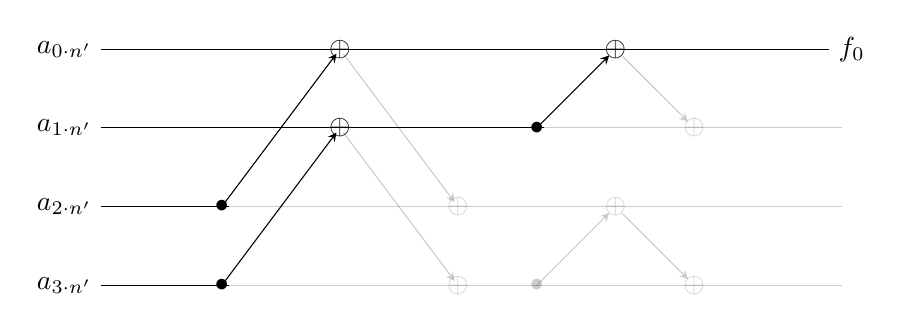
\begin{tikzpicture}
            \node (in4) at (0,3) {$a_{0\cdot n^\prime}$};
            \node (in3) at (0,2) {$a_{1\cdot n^\prime}$};
            \node (in2) at (0,1) {$a_{2\cdot n^\prime}$};
            \node (in1) at (0,0) {$a_{3\cdot n^\prime}$};
            \node (truncout4) at (10,3) {$f_0$};
            \node (truncout3) at (6,2) {};
            \node (truncout2) at (2,1) {};
            \node (truncout1) at (2,0) {};
            \node (out3) at (10,2) {};
            \node (out2) at (10,1) {};
            \node (out1) at (10,0) {};


            \node(m1) at (2, 0) {$\bullet$};
            \node(m2) at (2, 1) {$\bullet$};
            \node(m3) at (6, 2) {$\bullet$};
            \node[opacity=0.2](m4) at (6, 0) {$\bullet$};
            \node[opacity=0.2](a1) at (5, 0) {$\oplus$};
            \node[opacity=0.2](a2) at (5, 1) {$\oplus$};
            \node[opacity=0.2](a3) at (8, 2) {$\oplus$};
            \node[opacity=0.2](a4) at (8, 0) {$\oplus$};
            \node(b1) at (3.5, 2) {$\oplus$};
            \node(b2) at (3.5, 3) {$\oplus$};;
            \node(b3) at (7, 3) {$\oplus$};
            \node(b4)[opacity=0.2] at (7, 1) {$\oplus$};

            

            \draw[-, shorten >=-6pt] (in1) -- (truncout1);
            \draw[-, shorten >=-6pt] (in2) -- (truncout2);
            \draw[-, shorten >=-6pt] (in3) -- (truncout3);
            \draw[-, opacity=0.2, shorten <=-6pt] (truncout1) -- (out1);
            \draw[-, opacity=0.2, shorten <=-6pt] (truncout2) -- (out2);
            \draw[-, opacity=0.2, shorten <=-6pt] (truncout3) -- (out3);
            \draw[-] (in4) -- (truncout4);

            \draw[-stealth, shorten >=-6.5pt] (m1.center) -- (b1);
            \draw[-stealth, shorten >=-6.5pt, shorten <=-6.5pt, opacity=0.2] (b1) -- (a1);
            \draw[-stealth, shorten >=-6.5pt] (m2.center) -- (b2);
            \draw[-stealth, shorten >=-6.5pt, shorten <=-6.5pt, opacity=0.2] (b2) -- (a2);
            \draw[-stealth, shorten >=-6.5pt] (m3.center) -- (b3);
            \draw[-stealth, shorten >=-6.5pt, shorten <=-6.5pt, opacity=0.2] (b3) -- (a3);
            \draw[-stealth, shorten >=-6.5pt, opacity=0.2] (m4.center) -- (b4);
            \draw[-stealth, shorten >=-6.5pt, shorten <=-6.5pt, opacity=0.2] (b4) -- (a4);


        \end{tikzpicture}
    \end{center}
    \caption{A 2-layer Truncated FFT}
    \label{fig:trunc-fft} 
\end{figure}
            Because of the recursive nature of the vanishing polynomial, we can rewrite the result above as:
            \begin{equation*}
                f_0 = a_{0\cdot n^\prime} + v_{m/2-1}\cdot a_{1\cdot n^\prime} + v_{m/2-2}\cdot a_{2\cdot n^\prime} + v_{m/2-2}\cdot a_{3\cdot n^\prime} 
            \end{equation*}
            where the multipliers are independent of $l$ for a fixed $m$. Since the multipliers are in $\mathds{F}_{2^m}$ the output $f_0$ is in the same field, 
            thus not requiring the computation of the remaining values.
        \end{example}

    After this step, we can finally carry out the remaining butterfly computations, evaluating the encoded polynomials at the points in $\mathbf{S}$.

    \begin{figure}[H]
    \caption{A size-8 FFT}
    \begin{center}
        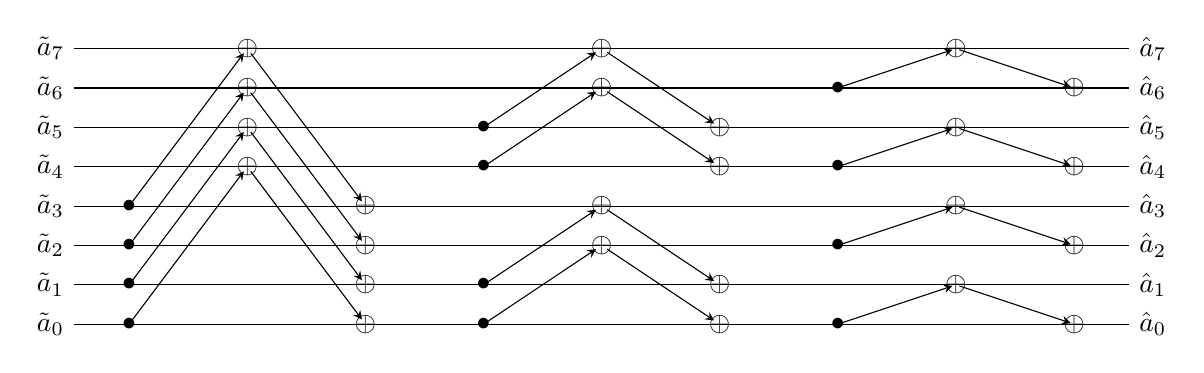
\begin{tikzpicture}[scale=0.5]
            \node (in8) at (0,7) {$\tilde{a}_7$};
            \node (in7) at (0,6) {$\tilde{a}_6$};
            \node (in6) at (0,5) {$\tilde{a}_5$};
            \node (in5) at (0,4) {$\tilde{a}_4$};
            \node (in4) at (0,3) {$\tilde{a}_3$};
            \node (in3) at (0,2) {$\tilde{a}_2$};
            \node (in2) at (0,1) {$\tilde{a}_1$};
            \node (in1) at (0,0) {$\tilde{a}_0$};
            \node (out8) at (28,7) {$\hat{a}_7$};
            \node (out7) at (28,6) {$\hat{a}_6$};
            \node (out6) at (28,5) {$\hat{a}_5$};
            \node (out5) at (28,4) {$\hat{a}_4$};
            \node (out4) at (28,3) {$\hat{a}_3$};
            \node (out3) at (28,2) {$\hat{a}_2$};
            \node (out2) at (28,1) {$\hat{a}_1$};
            \node (out1) at (28,0) {$\hat{a}_0$};


            \node(m1) at (2, 0) {$\bullet$};
            \node(m2) at (11, 0) {$\bullet$};
            \node(m3) at (20, 0) {$\bullet$};
            \node(m4) at (2, 1) {$\bullet$};
            \node(m5) at (11, 1) {$\bullet$};
            \node(m6) at (20, 2) {$\bullet$};
            \node(m7) at (2, 2) {$\bullet$};
            \node(m8) at (11, 4) {$\bullet$};
            \node(m9) at (20, 4) {$\bullet$};
            \node(m10) at (2, 3) {$\bullet$};
            \node(m11) at (11, 5) {$\bullet$};
            \node(m12) at (20, 6) {$\bullet$};

            \node(a1) at (8, 0) {$\oplus$};
            \node(a2) at (17, 0) {$\oplus$};
            \node(a3) at (26, 0) {$\oplus$};
            \node(a4) at (8, 1) {$\oplus$};
            \node(a5) at (17, 1) {$\oplus$};
            \node(a6) at (26, 2) {$\oplus$};
            \node(a7) at (8, 2) {$\oplus$};
            \node(a8) at (17, 4) {$\oplus$};
            \node(a9) at (26, 4) {$\oplus$};
            \node(a10) at (8, 3) {$\oplus$};
            \node(a11) at (17, 5) {$\oplus$};
            \node(a12) at (26, 6) {$\oplus$};

            \node(b1) at (5, 4) {$\oplus$};
            \node(b2) at (14, 2) {$\oplus$};
            \node(b3) at (23, 1) {$\oplus$};
            \node(b4) at (5, 5) {$\oplus$};
            \node(b5) at (14, 3) {$\oplus$};
            \node(b6) at (23, 3) {$\oplus$};
            \node(b7) at (5, 6) {$\oplus$};
            \node(b8) at (14, 6) {$\oplus$};
            \node(b9) at (23, 5) {$\oplus$};
            \node(b10) at (5, 7) {$\oplus$};
            \node(b11) at (14, 7) {$\oplus$};
            \node(b12) at (23, 7) {$\oplus$};

            \draw[-] (in1) -- (out1);
            \draw[-] (in2) -- (out2);
            \draw[-] (in3) -- (out3);
            \draw[-] (in4) -- (out4);
            \draw[-] (in5) -- (out5);
            \draw[-] (in6) -- (out6);
            \draw[-] (in7) -- (out7);
            \draw[-] (in8) -- (out8);

            \draw[-stealth, shorten >=-6.5pt] (m1.center) -- (b1);
            \draw[-stealth, shorten >=-6.5pt, shorten <=-6.5pt] (b1) -- (a1);
            \draw[-stealth, shorten >=-6.5pt] (m2.center) -- (b2);
            \draw[-stealth, shorten >=-6.5pt, shorten <=-6.5pt] (b2) -- (a2);
            \draw[-stealth, shorten >=-6.5pt] (m3.center) -- (b3);
            \draw[-stealth, shorten >=-6.5pt, shorten <=-6.5pt] (b3) -- (a3);
            \draw[-stealth, shorten >=-6.5pt] (m4.center) -- (b4);
            \draw[-stealth, shorten >=-6.5pt, shorten <=-6.5pt] (b4) -- (a4);
            \draw[-stealth, shorten >=-6.5pt] (m5.center) -- (b5);
            \draw[-stealth, shorten >=-6.5pt, shorten <=-6.5pt] (b5) -- (a5);
            \draw[-stealth, shorten >=-6.5pt] (m6.center) -- (b6);
            \draw[-stealth, shorten >=-6.5pt, shorten <=-6.5pt] (b6) -- (a6);
            \draw[-stealth, shorten >=-6.5pt] (m7.center) -- (b7);
            \draw[-stealth, shorten >=-6.5pt, shorten <=-6.5pt] (b7) -- (a7);
            \draw[-stealth, shorten >=-6.5pt] (m8.center) -- (b8);
            \draw[-stealth, shorten >=-6.5pt, shorten <=-6.5pt] (b8) -- (a8);
            \draw[-stealth, shorten >=-6.5pt] (m9.center) -- (b9);
            \draw[-stealth, shorten >=-6.5pt, shorten <=-6.5pt] (b9) -- (a9);
            \draw[-stealth, shorten >=-6.5pt] (m10.center) -- (b10);
            \draw[-stealth, shorten >=-6.5pt, shorten <=-6.5pt] (b10) -- (a10);
            \draw[-stealth, shorten >=-6.5pt] (m11.center) -- (b11);
            \draw[-stealth, shorten >=-6.5pt, shorten <=-6.5pt] (b11) -- (a11);
            \draw[-stealth, shorten >=-6.5pt] (m12.center) -- (b12);
            \draw[-stealth, shorten >=-6.5pt, shorten <=-6.5pt] (b12) -- (a12);
        \end{tikzpicture}
    \end{center}
    \label{fig:fft-full} 
\end{figure}

    Similarly to other FFT-based approaches, in order to perform the multiplication of two polynomials we have to apply the FFT on the inputs, 
    multiply the samples pointwise and then apply the inverse FFT; the summary of this procedure is shown in Algorithm~\ref{alg:fafft}.

    \begin{algorithm2e}[H]
        \caption{Frobenius Additive FFT Multiplication}
        \label{alg:fafft}
        \KwIn{$A(x) = a_0 + a_1x + \cdots + a_{n-1}x^{n-1} \in \mathds{F}_2[x]_{<n}$,\newline
            $B(x) = b_0 + b_1x + \cdots + b_{n-1}x^{n-1} \in \mathds{F}_2[x]_{<n}$}
        \KwOut{$C(x) = c_0 + c_1x + \cdots + c_{n-1}x^{n-1} = A(x)\cdot B(x) \mod (x^n+1) \in \mathds{F}_2[x]_{<n}$}
        \SetKwFunction{fftmul}{\textsc{MultFAFFT}}
        \SetKwProg{Fn}{Function}{}{}

        \Fn{\fftmul{$A(X), B(X)$}}{
            $\bar{A}(X) \gets \texttt{\textsc{BasisCvt}}(A(x))$\tcp*{$\in \mathds{F}_2[x]_{<n}$}
            $\bar{B}(X) \gets \texttt{\textsc{BasisCvt}}(B(x))$\tcp*{$\in \mathds{F}_2[x]_{<n}$}
            $\tilde{A}(X) \gets \texttt{\textsc{Encode}}(\bar{A}(X))$\tcp*{$\in \mathds{F}_{2^m}[x]_{<n^\prime}$}
            $\tilde{B}(X) \gets \texttt{\textsc{Encode}}(\bar{B}(X))$\tcp*{$\in \mathds{F}_{2^m}[x]_{<n^\prime}$}
            $[\hat{a}_1, \cdots, \hat{a}_{n^\prime}] \gets \texttt{\textsc{Butterflies}}(\tilde{A}(X), \mathbf{S})$\tcp*{$\in \mathds{F}_{2^m}^{n^\prime}$}
            $[\hat{b}_1, \cdots, \hat{b}_{n^\prime}] \gets \texttt{\textsc{Butterflies}}(\tilde{B}(X), \mathbf{S})$\tcp*{$\in \mathds{F}_{2^m}^{n^\prime}$}
            $\hat{C} = [\hat{c}_1, \cdots, \hat{c}_{n^\prime}] \gets [\hat{a}_1\cdot \hat{b}_1, \cdots, \hat{a}_{n^\prime}\cdot \hat{b}_{n^\prime}]$\;
            $\tilde{C}(X) \gets \texttt{\textsc{Butterflies}}^{-1}(\hat{C}, \mathbf{S})$\tcp*{$\in \mathds{F}_{2^m}[x]_{<n^\prime}$}
            $\bar{C}(X) \gets \texttt{\textsc{Decode}}(\tilde{C}(X))$\tcp*{$\in \mathds{F}_2[x]_{<n}$}
            $C(x) \gets \texttt{\textsc{BasisCvt}}^{-1}(\bar{C}(X))$\tcp*{$\in \mathds{F}_2[x]_{<n}$}
            \KwRet{$C(x) \mod (x^n+1)$}
        }
    \end{algorithm2e}

